\chapter{Números cuánticos y configuraciones electrónicas}\label{ch:b1:quantum-numbers}

Llénese un tubo de vidrio con hidrógeno a baja presión, hágase pasar por
él una descarga eléctrica y mírese su resplandor rosado a través de un
prisma. La luz no se abre en un arcoíris: se separa en cuatro líneas
nítidas --- una roja, una verde azulada y dos violetas --- y nada entre
ellas. Un sólido caliente emite a todas las longitudes de onda; un átomo
de hidrógeno solo emite unas pocas. La explicación, hallada entre 1913 y
1926, es que la energía de un electrón en un átomo no puede tomar
cualquier valor: está \emph{cuantizada}. Este capítulo enuncia las reglas
de esa cuantización tal como las usa el químico --- cuatro números
cuánticos y tres reglas de llenado --- y las convierte en la
\omterm{def:b1:quantum-numbers:configuration}{configuración electrónica} de todo átomo y de todo ion, la clave de la
tabla periódica del capítulo siguiente.

\begin{recall}
El libro 1 (año 10) colocó los electrones de los veinte primeros
elementos en capas y \omterm{def:b1:quantum-numbers:orbital}{subcapas}, 1s, 2s, 2p, 3s, 3p, y llamó \omterm{def:b1:quantum-numbers:configuration}{electrones de
valencia} a los de la capa más externa. De la física se da por conocido
que la luz de longitud de onda $\lambda$ está formada por fotones de
energía
$E = h\nu = hc/\lambda$, donde $h$ es la constante de Planck y $c$ la
velocidad de la luz.
\end{recall}

\begin{omfigure}

\includegraphics[width=0.62\linewidth]{images/book2/ai/b1-01-street-lamps.jpg}

{\small Farolas de vapor de sodio a baja presión. Su luz es casi una sola
línea amarillo anaranjada: como el hidrógeno, un átomo de sodio excitado
solo emite fotones de unas pocas energías precisas.}
\end{omfigure}

\section{Energías cuantizadas: el espectro del hidrógeno}

\begin{definition}[Nivel de energía, estado fundamental, estado excitado]\label{def:b1:quantum-numbers:energy-level}
La energía de un electrón ligado a un átomo solo puede tomar ciertos
valores, los \emph{niveles de energía}\index{nivel de energia@nivel de energía} del átomo. El cero
de energía se toma cuando el electrón está en reposo a distancia infinita
del núcleo (el átomo está ionizado), de modo que todo nivel de un
electrón ligado es negativo. El nivel más bajo es el \emph{estado
fundamental}\index{estado fundamental}; cualquier otro nivel es un
\emph{estado excitado}\index{estado excitado}.
\end{definition}

Un átomo pasa de un \omterm{def:b1:quantum-numbers:energy-level}{nivel de energía} $E_{\text{sup}}$ a un nivel más bajo
$E_{\text{inf}}$ emitiendo un fotón, y del nivel más bajo al más alto
absorbiendo uno, de energía
\[
  h\nu = \frac{hc}{\lambda} = E_{\text{sup}} - E_{\text{inf}} .
\]
Un espectro de líneas es, por tanto, una imagen de las diferencias entre
los niveles.

\begin{theorem}[Niveles de energía del átomo de hidrógeno]\label{thm:b1:quantum-numbers:levels}
Los \omterm{def:b1:quantum-numbers:energy-level}{niveles de energía} del átomo de hidrógeno son
\[
  E_n = -\frac{E_R}{n^2}, \qquad n = 1, 2, 3, \dots,
  \qquad E_R = \qty{13.6}{eV},
\]
donde $E_R$ es la energía de Rydberg (corregida por el movimiento del
núcleo). El \omterm{def:b1:quantum-numbers:energy-level}{estado fundamental} es $E_1 = \qty{-13.6}{eV}$ y la energía de
ionización del átomo es $E_R$.
% ledger: const:RyhcEV, ie:H (13.598 eV; levels computed in
% figdata/bachelor-1/hydrogen-levels.py)
\end{theorem}
\admitted

\begin{remark}[De dónde sale la fórmula]\label{rem:b1:quantum-numbers:schrodinger}
La fórmula se obtiene al resolver la ecuación de Schrödinger del electrón
en el campo del protón; la resolución, y las formas de las funciones de
onda que proporciona, se deducen en el volumen del segundo año. Niels Bohr
había obtenido los mismos niveles en 1913 con un modelo más sencillo de
órbitas circulares, hoy abandonado.
\end{remark}

\begin{proposition}[La fórmula de Rydberg]\label{prop:b1:quantum-numbers:rydberg}
Las líneas que emite el hidrógeno tienen longitudes de onda dadas por
\[
  \frac{1}{\lambda} = R_H\left(\frac{1}{n_1^2} - \frac{1}{n_2^2}\right),
  \qquad n_2 > n_1 \ge 1, \qquad R_H = \frac{E_R}{hc},
\]
para la transición del nivel $n_2$ al nivel inferior $n_1$. Las líneas que
terminan en un mismo nivel $n_1$ forman una \emph{serie}: la de Lyman para
$n_1 = 1$ (ultravioleta), la de Balmer para $n_1 = 2$ (visible) y la de
Paschen para $n_1 = 3$ (infrarrojo).
\end{proposition}

\begin{proof}
El fotón se lleva la energía que pierde el átomo:
$hc/\lambda = E_{n_2} - E_{n_1} = -E_R/n_2^2 + E_R/n_1^2
= E_R\,(1/n_1^2 - 1/n_2^2)$. Al dividir por $hc$ se obtiene la fórmula.
\end{proof}

\begin{example}[La línea roja del hidrógeno]\label{ex:b1:quantum-numbers:halpha}
Para la transición $3 \to 2$: $\Delta E = 13.6\,(1/4 - 1/9) =
\qty{1.89}{eV}$. Con $hc = \qty{1240}{eV.nm}$ (a partir de los valores de
$h$, $c$ y $e$), $\lambda = 1240/1.89 = \qty{656}{nm}$: la línea roja.
Las demás líneas de Balmer, $4 \to 2$, $5 \to 2$ y $6 \to 2$, caen en 486,
434 y \qty{410}{nm}; la siguiente, $7 \to 2$ en \qty{397}{nm}, está ya en
el ultravioleta. Las longitudes de onda medidas, 656.3, 486.1, 434.0 y
\qty{410.2}{nm}, concuerdan mejor que en una parte en dos mil; la pequeña
diferencia restante se debe a que se miden en el aire y no en el vacío.
% ledger: asd:Halpha, asd:Hbeta, asd:Hgamma, asd:Hdelta (computed values
% in figdata/out/bachelor-1-hydrogen-levels-balmer.dat)
\end{example}

\begin{omfigure}
\begin{tikzpicture}
\begin{axis}[
  width=0.62\linewidth, height=7.2cm,
  xmin=0, xmax=10, ymin=-14.5, ymax=0.6,
  axis x line=none, axis y line=left,
  ylabel={energía (eV)}, ytick={-14,-12,-10,-8,-6,-4,-2,0},
  tick label style={font=\small}, label style={font=\small},
  clip=false]
\pgfplotsinvokeforeach{-13.598,-3.400,-1.511,-0.850,-0.544}{
  \draw[black!70, line width=0.7pt] (axis cs:0.3,#1) -- (axis cs:9.6,#1);}
\draw[black!40, dashed] (axis cs:0.3,0) -- (axis cs:9.6,0);
\node[font=\small, anchor=west] at (axis cs:9.7,-13.598) {$n = 1$};
\node[font=\small, anchor=west] at (axis cs:9.7,-3.400) {$n = 2$};
\node[font=\small, anchor=west] at (axis cs:9.7,-1.511) {$n = 3$};
\node[font=\small, anchor=south west] at (axis cs:9.7,0.05) {$n \to \infty$};
% Lyman
\draw[-{Stealth}, violet!70!black, thick] (axis cs:1.0,-3.400) -- (axis cs:1.0,-13.598);
\draw[-{Stealth}, violet!70!black, thick] (axis cs:1.6,-1.511) -- (axis cs:1.6,-13.598);
\draw[-{Stealth}, violet!70!black, thick] (axis cs:2.2,-0.850) -- (axis cs:2.2,-13.598);
\node[font=\small, violet!70!black, anchor=west] at (axis cs:2.4,-9) {Lyman};
% Balmer
\draw[-{Stealth}, red!80!black, thick] (axis cs:4.4,-1.511) -- (axis cs:4.4,-3.400);
\draw[-{Stealth}, teal!80!black, thick] (axis cs:5.0,-0.850) -- (axis cs:5.0,-3.400);
\draw[-{Stealth}, blue!80!black, thick] (axis cs:5.6,-0.544) -- (axis cs:5.6,-3.400);
\node[font=\small, anchor=north] at (axis cs:5.0,-3.6) {Balmer};
% Paschen
\draw[-{Stealth}, black!60, thick] (axis cs:7.8,-0.850) -- (axis cs:7.8,-1.511);
\draw[-{Stealth}, black!60, thick] (axis cs:8.4,-0.544) -- (axis cs:8.4,-1.511);
\node[font=\small, anchor=north] at (axis cs:8.1,-1.7) {Paschen};
\end{axis}
\end{tikzpicture}

{\small Los \omterm{def:b1:quantum-numbers:energy-level}{niveles de energía} del hidrógeno, $E_n = -\qty{13.6}{eV}/n^2$,
dibujados a escala (calculados a partir de la constante de Rydberg); los
niveles $n = 4,
5, \dots$ se apiñan por debajo de cero. Cada flecha es un
fotón emitido; las flechas que terminan en un mismo nivel forman una serie.}
\end{omfigure}

\begin{omfigure}
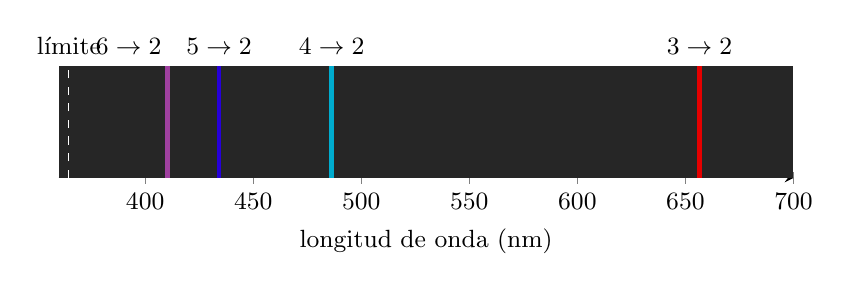
\begin{tikzpicture}
\begin{axis}[
  width=0.9\linewidth, height=3.0cm,
  xmin=360, xmax=700, ymin=0, ymax=1,
  axis x line=bottom, axis y line=none,
  xlabel={longitud de onda (nm)}, xtick={400,450,500,550,600,650,700},
  tick label style={font=\small}, label style={font=\small},
  clip=false]
\fill[black!85] (axis cs:360,0) rectangle (axis cs:700,1);
% line positions: figdata/out/bachelor-1-hydrogen-levels-balmer.dat
\draw[line width=1.6pt, red!90!black] (axis cs:656.5,0) -- (axis cs:656.5,1);
\draw[line width=1.6pt, cyan!80!green] (axis cs:486.3,0) -- (axis cs:486.3,1);
\draw[line width=1.6pt, blue!70!violet] (axis cs:434.2,0) -- (axis cs:434.2,1);
\draw[line width=1.6pt, violet!75] (axis cs:410.3,0) -- (axis cs:410.3,1);
\draw[white, dashed] (axis cs:364.7,0) -- (axis cs:364.7,1);
\node[font=\small, anchor=south] at (axis cs:364.7,1.02) {límite};
\node[font=\small, anchor=south] at (axis cs:656.5,1.02) {$3\to2$};
\node[font=\small, anchor=south] at (axis cs:486.3,1.02) {$4\to2$};
\node[font=\small, anchor=south] at (axis cs:434.2,1.02) {$5\to2$};
\node[font=\small, anchor=south east] at (axis cs:412,1.02) {$6\to2$};
\end{axis}
\end{tikzpicture}

{\small Las líneas de Balmer calculadas con la fórmula de Rydberg
(longitudes de onda en el vacío), sobre la banda visible. Otras líneas se
apiñan hacia el límite de la serie, en \qty{364.7}{nm}, en el ultravioleta.}
\end{omfigure}

\begin{history}[El átomo de Bohr, 1913]
En 1913, Niels Bohr, un físico danés de 28 años que trabajaba en
Mánchester, propuso que el electrón del hidrógeno solo podía girar
alrededor del núcleo en ciertas órbitas, y que la luz se emitía cuando
saltaba de una órbita a otra más baja. Su modelo daba exactamente las
líneas de Balmer, y el valor de la constante de Rydberg a partir de $h$,
$e$ y la masa del electrón. Las órbitas no sobrevivieron a la mecánica
cuántica de 1925--1926, pero los niveles cuantizados sí. Bohr recibió el
Premio Nobel de Física en 1922.
\end{history}

\begin{omfigure}
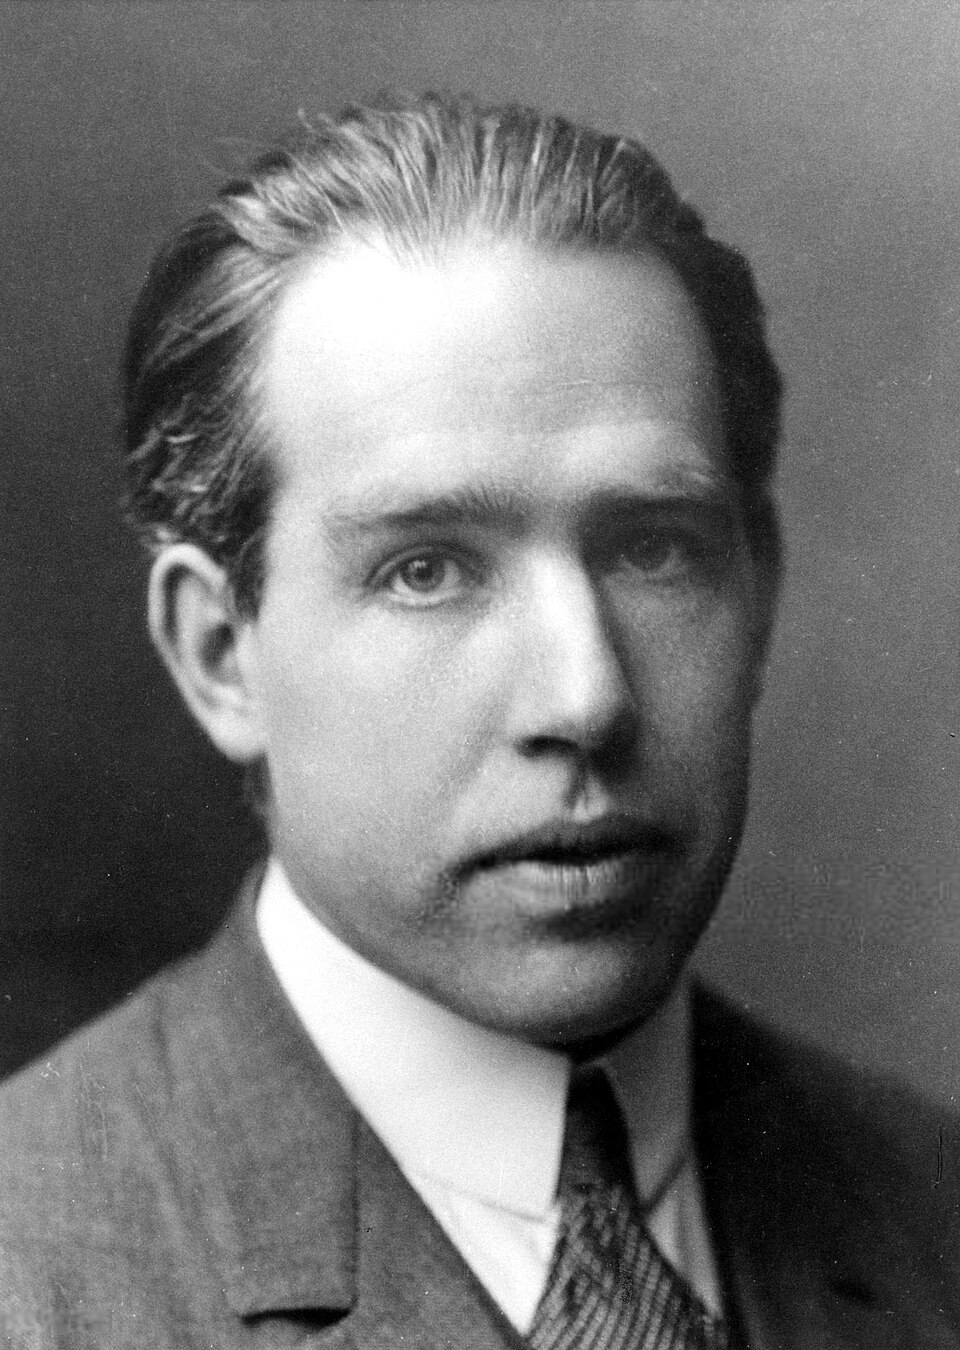
\includegraphics[width=0.26\linewidth]{images/book2/bohr.jpg}

{\small Niels Bohr (1885--1962), hacia 1922.}
\end{omfigure}

\section{Cuatro números cuánticos}

En un átomo con muchos electrones las energías ya no vienen dadas por una
sola fórmula, pero cada electrón sigue descrito por un pequeño conjunto
de enteros, sus números cuánticos.

\begin{definition}[Números cuánticos]\label{def:b1:quantum-numbers:quantum-number}
El estado de un electrón en un átomo se designa con cuatro números:
\begin{itemize}
  \item el \emph{número cuántico principal}\index{numero cuantico principal@número cuántico principal}
        $n = 1, 2, 3, \dots$, que fija sobre todo la energía y el tamaño;
  \item el \emph{número cuántico azimutal}\index{numero cuantico azimutal@número cuántico azimutal}
        (o número cuántico secundario) $l = 0, 1, \dots, n-1$, que fija
        la forma; $l = 0, 1, 2, 3$ se escriben s, p, d, f;
  \item el \emph{número cuántico magnético}\index{numero cuantico magnetico@número cuántico magnético}
        $m_l = -l, -l+1, \dots, l$, que fija la orientación ($2l + 1$
        valores);
  \item el \emph{número cuántico de espín}\index{numero cuantico de espin@número cuántico de espín}
        $m_s = +\tfrac12$ o $-\tfrac12$, una propiedad intrínseca del
        electrón, que se dibuja como una flecha hacia arriba o hacia abajo.
\end{itemize}
\end{definition}

\begin{definition}[Orbital atómico, capa, subcapa]\label{def:b1:quantum-numbers:orbital}
Un \emph{orbital atómico}\index{orbital atomico@orbital atómico} es el estado de un electrón
designado por los tres números $(n, l, m_l)$; se dibuja como una casilla,
\omorbs{}. Los orbitales con el mismo $n$ forman una \emph{capa
electrónica}\index{capa electronica@capa electrónica}; los que tienen el mismo $n$ y el mismo $l$ forman una
\emph{subcapa}\index{subcapa}, que se nombra con $n$ y la letra de $l$:
2p es la subcapa $n = 2$, $l = 1$, formada por tres orbitales
($m_l = -1, 0, 1$).
\end{definition}

\begin{remark}[Formas]\label{rem:b1:quantum-numbers:shapes}
Un orbital s es esférico; un orbital p tiene dos lóbulos a lo largo de un
eje, y los tres orbitales 2p apuntan según $x$, $y$ y $z$. La descripción
matemática de estas formas --- funciones de onda, sus partes radial y
angular, sus nodos --- corresponde al volumen del segundo año. En este
libro, un orbital es una casilla que admite como máximo dos electrones.
\end{remark}

\begin{proposition}[Capacidad de una subcapa y de una capa]\label{prop:b1:quantum-numbers:capacity}
Una \omterm{def:b1:quantum-numbers:orbital}{subcapa} de número azimutal $l$ contiene $2l + 1$ orbitales y admite
$2(2l + 1)$ electrones: 2 en s, 6 en p, 10 en d, 14 en f. La capa $n$
contiene $n^2$ orbitales y admite $2n^2$ electrones.
\end{proposition}

\begin{proof}
Para un $l$ dado, $m_l$ toma los $2l + 1$ valores de $-l$ a $l$, y cada
orbital admite dos electrones de espines opuestos (\cref{prop:b1:quantum-numbers:pauli}
más abajo). Para un $n$ dado, $l$ va de $0$ a $n - 1$, de modo que el
número de orbitales es
\[
  \sum_{l=0}^{n-1} (2l+1) = 2\,\frac{(n-1)n}{2} + n = n^2 ,
\]
y el número de electrones es $2n^2$: 2, 8, 18, 32 para $n = 1$ a 4.
\end{proof}

\begin{example}[La tercera capa]\label{ex:b1:quantum-numbers:third}
Para $n = 3$: $l = 0$ (3s, un orbital), $l = 1$ (3p, tres orbitales),
$l = 2$ (3d, cinco orbitales, $m_l = -2, \dots, 2$): nueve orbitales y
hasta 18 electrones. Un electrón 3d tiene, por ejemplo, los números
cuánticos $(3, 2, -1, +\tfrac12)$.
\end{example}

\section{Construcción de las configuraciones}

\begin{definition}[Configuración electrónica]\label{def:b1:quantum-numbers:configuration}
La \emph{configuración electrónica}\index{configuracion electronica@configuración electrónica} de un
átomo o de un ion es la lista de sus \omterm{def:b1:quantum-numbers:orbital}{subcapas} ocupadas con el número de
electrones de cada una escrito como exponente: $1\text{s}^2 2\text{s}^2
2\text{p}^4$ para el oxígeno. Los electrones del $n$ más alto, junto con
los de una \omterm{def:b1:quantum-numbers:orbital}{subcapa} d o f incompleta, son los \emph{electrones de
valencia}\index{electrones de valencia}; los demás son los \emph{electrones
internos}\index{electrones internos}. Una configuración se abrevia
escribiendo entre corchetes la configuración del gas noble anterior:
el oxígeno es $[\ce{He}]\,2\text{s}^2 2\text{p}^4$.
\end{definition}

Tres reglas dan la configuración del \omterm{def:b1:quantum-numbers:energy-level}{estado fundamental}.

\begin{proposition}[Principio de exclusión de Pauli]\label{prop:b1:quantum-numbers:pauli}
Dos electrones de un mismo átomo nunca tienen los mismos cuatro números
cuánticos. Por tanto, un orbital admite como máximo dos electrones, y
entonces de espines opuestos: \omorbs{ud}.
\end{proposition}
\admitted

\begin{proposition}[Regla de Klechkowski]\label{prop:b1:quantum-numbers:klechkowski}
En el \omterm{def:b1:quantum-numbers:energy-level}{estado fundamental} de un átomo neutro, las \omterm{def:b1:quantum-numbers:orbital}{subcapas} se llenan en el
orden de $n + l$ creciente y, a igual $n + l$, por orden creciente de
$n$:
\[
  1\text{s},\ 2\text{s},\ 2\text{p},\ 3\text{s},\ 3\text{p},\ 4\text{s},\
  3\text{d},\ 4\text{p},\ 5\text{s},\ 4\text{d},\ 5\text{p},\ 6\text{s},\
  4\text{f},\ 5\text{d},\ 6\text{p},\ 7\text{s},\ 5\text{f},\ 6\text{d},\
  7\text{p}.
\]
\end{proposition}
\admitted

\begin{remark}[Una regla empírica]\label{rem:b1:quantum-numbers:klech-empirical}
La regla de Klechkowski (también llamada regla de Madelung) resume las
configuraciones observadas; no es una ley: describe el orden en que se
llenan las \omterm{def:b1:quantum-numbers:orbital}{subcapas} a medida que aumenta la carga nuclear. En un átomo con
muchos electrones, los electrones se repelen entre sí, de modo que la
energía de una \omterm{def:b1:quantum-numbers:orbital}{subcapa} depende de $l$ además de $n$: un electrón 4s, que
pasa parte de su tiempo cerca del núcleo, acaba por debajo de 3d en el
potasio y el calcio.
\end{remark}

\begin{omfigure}
\begin{tikzpicture}[font=\small, x=1.25cm, y=0.72cm]
  \foreach \n in {1,...,7} {
    \foreach \l/\s in {0/s,1/p,2/d,3/f} {
      \pgfmathtruncatemacro\ok{(\l<\n) && (\n+\l<=8)}
      \ifnum\ok=1
        \node[draw=black!50, rounded corners=2pt, minimum width=0.85cm,
          minimum height=0.5cm, fill=white] (s\n\l) at (\l,-\n) {\n\s};
      \fi
    }
  }
  \begin{scope}[on background layer]
  \foreach \la/\na/\lb/\nb in {0/1/0/1, 0/2/0/2, 1/2/0/3, 1/3/0/4, 2/3/0/5,
      2/4/0/6, 3/4/0/7, 3/5/1/7} {
    \draw[-{Stealth}, omDef, thick, opacity=0.8]
      ($(\la,-\na)+(0.5,0.42)$) -- ($(\lb,-\nb)+(-0.5,-0.42)$);
  }
  \end{scope}
  \node[anchor=west, align=left, font=\small] at (4.0,-2.5) {síganse las flechas\\una tras otra,\\de izquierda a derecha};
\end{tikzpicture}

{\small El diagrama de Klechkowski. Las \omterm{def:b1:quantum-numbers:orbital}{subcapas} con el mismo $n + l$ están
sobre una misma diagonal; recorrer las diagonales en orden da el orden de
llenado
1s, 2s, 2p, 3s, 3p, 4s, 3d, 4p, 5s, \dots}
\end{omfigure}

\begin{proposition}[Regla de Hund]\label{prop:b1:quantum-numbers:hund}
Cuando los electrones de una \omterm{def:b1:quantum-numbers:orbital}{subcapa} pueden colocarse en varios orbitales
de la misma energía, el \omterm{def:b1:quantum-numbers:energy-level}{estado fundamental} tiene el mayor número de
espines \emph{paralelos}: los electrones ocupan orbitales distintos, con
el espín hacia arriba, antes de que ningún orbital se llene con dos.
\end{proposition}
\admitted

\begin{definition}[Electrón desapareado]\label{def:b1:quantum-numbers:unpaired}
Un \emph{electrón desapareado}\index{electron desapareado@electrón desapareado} es un electrón
solo en su orbital. Una especie con electrones desapareados es atraída
por un imán (es paramagnética, una propiedad que se estudia en física).
\end{definition}

\begin{method}[Escribir una configuración del estado fundamental]\label{met:b1:quantum-numbers:configuration}
Para escribir la configuración de un átomo de número atómico $Z$:
\begin{enumerate}
  \item se colocan $Z$ electrones en las \omterm{def:b1:quantum-numbers:orbital}{subcapas} siguiendo el orden de
        Klechkowski, llenando cada \omterm{def:b1:quantum-numbers:orbital}{subcapa} (2, 6, 10, 14) antes de la
        siguiente;
  \item se escribe el resultado en orden de $n$ creciente (agrupando 3d
        con $n = 3$) y se abrevia con el núcleo del gas noble anterior;
  \item para la última \omterm{def:b1:quantum-numbers:orbital}{subcapa}, incompleta, se dibujan las casillas y se
        aplica la regla de Hund para contar los \omterm{def:b1:quantum-numbers:unpaired}{electrones desapareados}.
\end{enumerate}
\end{method}

\begin{example}[Carbono, nitrógeno, oxígeno, hierro]\label{ex:b1:quantum-numbers:examples}
El método da, para cuatro átomos:
\begin{center}
\begin{tabular}{lllc}
\hline
átomo & configuración & última \omterm{def:b1:quantum-numbers:orbital}{subcapa} & desapareados \\
\hline
\ce{C} ($Z = 6$) & $[\ce{He}]\,2\text{s}^2 2\text{p}^2$ & 2p: \omorbs{u,u,} & 2 \\
\ce{N} ($Z = 7$) & $[\ce{He}]\,2\text{s}^2 2\text{p}^3$ & 2p: \omorbs{u,u,u} & 3 \\
\ce{O} ($Z = 8$) & $[\ce{He}]\,2\text{s}^2 2\text{p}^4$ & 2p: \omorbs{ud,u,u} & 2 \\
\ce{Fe} ($Z = 26$) & $[\ce{Ar}]\,3\text{d}^6 4\text{s}^2$ & 3d: \omorbs{ud,u,u,u,u} & 4 \\
\hline
\end{tabular}
\end{center}
En el hierro, el orden de Klechkowski llena 4s ($Z = 19, 20$) antes que
3d ($Z = 21$ a 30); la configuración se escribe con 3d en primer lugar.
% ledger: gs:Fe
\end{example}

\begin{omfigure}
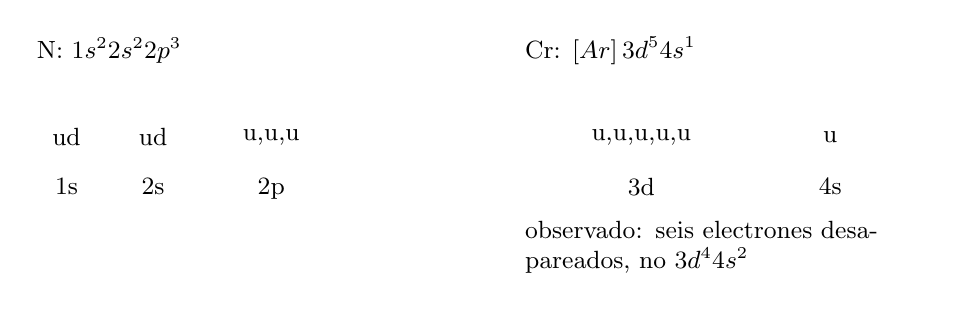
\begin{tikzpicture}[font=\small]
  \begin{scope}
    \node[anchor=west] at (0,2.4) {\ce{N}: $1\text{s}^2 2\text{s}^2 2\text{p}^3$};
    \node at (0.5,1.3) {\omorbs{ud}}; \node[below] at (0.5,0.9) {1s};
    \node at (1.6,1.3) {\omorbs{ud}}; \node[below] at (1.6,0.9) {2s};
    \node at (3.1,1.3) {\omorbs{u,u,u}}; \node[below] at (3.1,0.9) {2p};
  \end{scope}
  \begin{scope}[xshift=6.2cm]
    \node[anchor=west] at (0,2.4) {\ce{Cr}: $[\ce{Ar}]\,3\text{d}^5 4\text{s}^1$};
    \node at (1.6,1.3) {\omorbs{u,u,u,u,u}}; \node[below] at (1.6,0.9) {3d};
    \node at (4.0,1.3) {\omorbs{u}}; \node[below] at (4.0,0.9) {4s};
    \node[anchor=west, text width=5.0cm] at (0,-0.1) {observado: seis electrones desapareados, no $3\text{d}^4 4\text{s}^2$};
  \end{scope}
\end{tikzpicture}

{\small Casillas cuánticas. Cada casilla es un orbital; una flecha es un
electrón y su espín. El nitrógeno sigue la regla de Hund; el cromo es una
de las excepciones de la \cref{prop:b1:quantum-numbers:exceptions}.}
\end{omfigure}

\section{Iones, excepciones y forma de la tabla}

\begin{proposition}[Configuraciones de los iones]\label{prop:b1:quantum-numbers:ions}
Un anión monoatómico tiene la configuración del átomo con los electrones
adicionales colocados en los siguientes lugares del orden de Klechkowski;
un catión de un elemento de los grupos principales pierde los electrones
del $n$ más alto. Un catión de un metal de transición pierde sus
electrones $n$s \emph{antes} que sus electrones
$(n-1)$d: \ce{Fe^{2+}} es $[\ce{Ar}]\,3\text{d}^6$ y
\ce{Fe^{3+}} es $[\ce{Ar}]\,3\text{d}^5$, no $[\ce{Ar}]\,3\text{d}^4
4\text{s}^2$.
% ledger: gs:Fe2+, gs:Fe3+
\end{proposition}
\admitted

\begin{remark}[El orden de llenado no es el orden de extracción]\label{rem:b1:quantum-numbers:order}
4s se llena antes que 3d en el potasio y el calcio, y sin embargo se vacía
primero en los iones de los metales de transición. No hay contradicción:
el orden de las energías de las \omterm{def:b1:quantum-numbers:orbital}{subcapas} cambia con la carga nuclear y con
el número de electrones, y en un átomo o ion de un metal de transición la
\omterm{def:b1:quantum-numbers:orbital}{subcapa} 3d está por debajo de 4s. La regla de Klechkowski solo describe
átomos neutros.
\end{remark}

\begin{proposition}[Dos excepciones en la primera serie de transición]\label{prop:b1:quantum-numbers:exceptions}
Las configuraciones observadas del \omterm{def:b1:quantum-numbers:energy-level}{estado fundamental} del cromo y del
cobre son
\[
  \ce{Cr}: [\ce{Ar}]\,3\text{d}^5 4\text{s}^1, \qquad
  \ce{Cu}: [\ce{Ar}]\,3\text{d}^{10} 4\text{s}^1 ,
\]
en lugar de las $3\text{d}^4 4\text{s}^2$ y $3\text{d}^9 4\text{s}^2$
que predice la regla de Klechkowski: una \omterm{def:b1:quantum-numbers:orbital}{subcapa} d semillena o llena es
especialmente estable, y los niveles 4s y 3d están próximos.
% ledger: gs:Cr, gs:Cu
\end{proposition}

\begin{example}[El cobre y sus iones]\label{ex:b1:quantum-numbers:copper}
\ce{Cu} es $[\ce{Ar}]\,3\text{d}^{10} 4\text{s}^1$; \ce{Cu+} es
$[\ce{Ar}]\,3\text{d}^{10}$, sin ningún \omterm{def:b1:quantum-numbers:unpaired}{electrón desapareado}; \ce{Cu^{2+}}
es $[\ce{Ar}]\,3\text{d}^9$, con uno. \ce{Zn^{2+}}, $[\ce{Ar}]\,3\text{d}^{10}$,
no tiene ninguno.
% ledger: gs:Cu+, gs:Cu2+, gs:Zn2+
\end{example}

\begin{proposition}[Configuraciones y tabla periódica]\label{prop:b1:quantum-numbers:table}
El periodo $n$ de la tabla periódica empieza con el llenado de $n$s y
termina con el llenado de $n$p. Las \omterm{def:b1:quantum-numbers:orbital}{subcapas} que se llenan entre ambos
son, por la regla de Klechkowski, $(n-2)$f y $(n-1)$d. Por eso los
periodos contienen
$2, 8, 8, 18, 18, 32, 32$ elementos, y los gases nobles tienen $Z = 2, 10,
18, 36, 54, 86, 118$.
\end{proposition}

\begin{proof}
Los periodos 1 a 3 solo contienen $n$s (y $n$p para $n \ge 2$): $2$, y
luego $2 + 6 = 8$ dos veces. En los periodos 4 y 5 se añade $(n-1)$d:
$2 + 10 + 6 =
18$. En los periodos 6 y 7, además, $(n-2)$f: $2 + 14 + 10 + 6 = 32$. Los
gases nobles cierran cada periodo: $2$, $2 + 8 = 10$, $18$, $18 + 18 = 36$,
$54$, $54 + 32 = 86$, $118$.
\end{proof}

\begin{omfigure}
\omperiodictable[colour=blocks, legend]

{\small La tabla periódica coloreada según la última \omterm{def:b1:quantum-numbers:orbital}{subcapa} que se llena:
los bloques s, p, d y f. La anchura de cada bloque es la capacidad de su
\omterm{def:b1:quantum-numbers:orbital}{subcapa}, 2, 6, 10 y 14.}
\end{omfigure}

\section{Ejercicios}

\begin{exercise}[$\star$]\label{exo:b1:quantum-numbers:1}
¿Cuáles de estos conjuntos $(n, l, m_l, m_s)$ pueden describir un
electrón de un átomo? Justifíquese cada rechazo.
(a) $(2, 2, 0, +\tfrac12)$; (b) $(3, 1, -1, -\tfrac12)$;
(c) $(1, 0, 0, 0)$; (d) $(4, 3, -3, +\tfrac12)$; (e) $(3, 0, 1, -\tfrac12)$.
\end{exercise}

\begin{exercise}[$\star$]\label{exo:b1:quantum-numbers:2}
¿Cuántos orbitales, y como máximo cuántos electrones, hay en las
\omterm{def:b1:quantum-numbers:orbital}{subcapas} 3d, 4f y 5p, y en la capa $n = 2$?
\end{exercise}

\begin{exercise}[$\star$]\label{exo:b1:quantum-numbers:3}
Escríbanse las configuraciones del \omterm{def:b1:quantum-numbers:energy-level}{estado fundamental} de \ce{O}, \ce{P},
\ce{K}, \ce{Ca} y \ce{Br} ($Z = 8, 15, 19, 20, 35$), completas y
abreviadas, e indíquese el número de \omterm{def:b1:quantum-numbers:configuration}{electrones de valencia} de cada uno.
\end{exercise}

\begin{exercise}[$\star$]\label{exo:b1:quantum-numbers:4}
Dibújense las casillas cuánticas de las \omterm{def:b1:quantum-numbers:orbital}{subcapas} de valencia del
nitrógeno, el azufre y el cloro, y cuéntense sus \omterm{def:b1:quantum-numbers:unpaired}{electrones desapareados}.
\end{exercise}

\begin{exercise}[$\star\star$]\label{exo:b1:quantum-numbers:5}
Dense las configuraciones de \ce{Na+}, \ce{Mg^{2+}}, \ce{Al^{3+}}, \ce{F-},
\ce{O^{2-}}, \ce{Cl-}, \ce{S^{2-}} y \ce{Ca^{2+}}. ¿Con qué gas noble es
isoelectrónico cada uno?
\end{exercise}

\begin{exercise}[$\star\star$]\label{exo:b1:quantum-numbers:6}
Escríbanse las configuraciones de \ce{Ti^{2+}}, \ce{Mn^{2+}}, \ce{Co^{2+}},
\ce{Ni^{2+}} y \ce{Zn^{2+}} ($Z = 22, 25, 27, 28, 30$) e indíquese el
número de \omterm{def:b1:quantum-numbers:unpaired}{electrones desapareados} de cada uno.
\end{exercise}

\begin{exercise}[$\star\star$]\label{exo:b1:quantum-numbers:7}
Calcúlense la energía y la longitud de onda del fotón emitido en la
transición $4 \to 3$ del hidrógeno. ¿En qué zona del espectro se
encuentra? Tómense $E_R = \qty{13.6}{eV}$ y $hc = \qty{1240}{eV.nm}$.
\end{exercise}

\begin{exercise}[$\star\star$]\label{exo:b1:quantum-numbers:8}
Identifíquense los elementos cuya configuración del \omterm{def:b1:quantum-numbers:energy-level}{estado fundamental}
termina en
(a) $3\text{s}^2 3\text{p}^4$; (b) $4\text{s}^2 3\text{d}^{10} 4\text{p}^5$;
(c) $5\text{s}^1$; (d) $4\text{s}^2 3\text{d}^3$. Dense los cuatro
números cuánticos de un electrón de la última \omterm{def:b1:quantum-numbers:orbital}{subcapa} de (a).
\end{exercise}

\begin{exercise}[$\star\star$]\label{exo:b1:quantum-numbers:9}
Explíquese, con la regla de Klechkowski, por qué el decimonoveno electrón
del potasio entra en 4s y no en 3d, y por qué el periodo 3 contiene 8
elementos y no 18.
\end{exercise}

\begin{exercise}[$\star\star\star$]\label{exo:b1:quantum-numbers:10}
Un ion con un solo electrón y un núcleo de carga $Ze$ tiene los niveles
$E_n = -Z^2 E_R/n^2$ (se admite). Para \ce{He+} ($Z = 2$), calcúlense la
energía de ionización y la longitud de onda de la transición $2 \to 1$.
Compárese con el hidrógeno.
\end{exercise}

\begin{exercise}[$\star\star\star$]\label{exo:b1:quantum-numbers:11}
Dígase si cada configuración es un \omterm{def:b1:quantum-numbers:energy-level}{estado fundamental}, un \omterm{def:b1:quantum-numbers:energy-level}{estado excitado}
o imposible, y por qué: (a) $1\text{s}^2 2\text{s}^1 2\text{p}^1$;
(b) $1\text{s}^2 2\text{s}^2 2\text{p}^7$; (c) $1\text{s}^2 2\text{p}^2$;
(d) $[\ce{Ne}]\,3\text{s}^2 3\text{p}^3$; (e) $1\text{s}^3$.
\end{exercise}

\begin{exercise}[$\star\star\star$]\label{exo:b1:quantum-numbers:12}
Las sales de hierro(III) son atraídas por un imán con más fuerza que las
de hierro(II), y las de cinc, en absoluto. Ordénense \ce{Fe^{2+}},
\ce{Fe^{3+}}, \ce{Mn^{2+}}, \ce{Cu^{2+}} y \ce{Zn^{2+}} según su número
de \omterm{def:b1:quantum-numbers:unpaired}{electrones desapareados}, y explíquese la observación suponiendo que la
atracción crece con ese número.
\end{exercise}

\section{Problema: las líneas de una lámpara y un mundo con tres espines}

\begin{problem}[{Problema de fin de semana --- de las cuatro líneas de una
lámpara de hidrógeno a la longitud de los periodos, y cómo sería la tabla
si el electrón tuviera tres estados de espín}]
\label{pb:b1:quantum-numbers:1}
Tómense $E_R = \qty{13.6}{eV}$ y $hc = \qty{1240}{eV.nm}$ en todo el
problema. La banda visible va de unos 400 a \qty{700}{nm}.

\medskip
\noindent\textbf{Parte I --- La lámpara de hidrógeno.}
\begin{enumerate}
  \item Calcúlense las energías $E_1$ a $E_4$ del átomo de hidrógeno.
  \item Calcúlense la energía y la longitud de onda del fotón emitido en
        la transición $3 \to 2$. ¿De qué color es?
  \item Calcúlense las longitudes de onda de las transiciones $4 \to 2$,
        $5 \to 2$ y $6 \to 2$.
  \item ¿Por qué una lámpara de hidrógeno muestra exactamente cuatro
        líneas visibles? Calcúlese la longitud de onda de $7 \to 2$ para
        justificar la respuesta.
  \item Calcúlese el límite de la serie de Balmer.
  \item Calcúlese la longitud de onda de la primera línea de Lyman,
        $2 \to 1$. ¿Por qué no puede verse?
  \item ¿Cuál es la mayor longitud de onda de un fotón capaz de ionizar
        un átomo de hidrógeno en su \omterm{def:b1:quantum-numbers:energy-level}{estado fundamental}?
\end{enumerate}

\medskip
\noindent\textbf{Parte II --- Contar estados.}
\begin{enumerate}[resume]
  \item Enumérense los valores de $l$ y $m_l$ para $n = 3$; ¿cuántos
        orbitales contiene la capa?
  \item Demuéstrese que la capa $n$ admite $2n^2$ electrones; aplíquese a
        $n = 4$.
  \item Escríbase el orden de Klechkowski hasta 7p.
  \item Dedúzcanse las longitudes de los siete periodos.
  \item Explíquese por qué la \omterm{def:b1:quantum-numbers:orbital}{subcapa} 3d no aparece en el periodo 3.
  \item Dedúzcanse los números atómicos de los gases nobles.
\end{enumerate}

\medskip
\noindent\textbf{Parte III --- Los metales de transición.}
\begin{enumerate}[resume]
  \item Escríbase la configuración del hierro ($Z = 26$) y dibújense sus
        casillas 3d. ¿Cuántos \omterm{def:b1:quantum-numbers:unpaired}{electrones desapareados} tiene?
  \item Las mismas preguntas para \ce{Fe^{2+}} y \ce{Fe^{3+}}. ¿Cuál de
        los dos tiene una \omterm{def:b1:quantum-numbers:orbital}{subcapa} semillena?
  \item La configuración observada del cromo es $[\ce{Ar}]\,3\text{d}^5
        4\text{s}^1$. Compárese con la predicción y cuéntense los
        \omterm{def:b1:quantum-numbers:unpaired}{electrones desapareados} de cada una.
  \item Dense las configuraciones de \ce{Cu}, \ce{Cu+} y \ce{Cu^{2+}}.
  \item ¿Cuál de \ce{Cu+} y \ce{Cu^{2+}} tiene \omterm{def:b1:quantum-numbers:unpaired}{electrones desapareados}?
  \item Entre \ce{Sc^{3+}}, \ce{Ti^{3+}} y \ce{Mn^{2+}} ($Z = 21, 22, 25$),
        ¿cuál tiene más \omterm{def:b1:quantum-numbers:unpaired}{electrones desapareados}?
\end{enumerate}

\medskip
\noindent\textbf{Parte IV --- Un mundo con tres espines.}
Imagínese un universo en el que $n$, $l$ y $m_l$ obedecen las mismas
reglas que en el nuestro, el orden de Klechkowski no cambia y el
principio de exclusión se cumple, pero el número de espín $m_s$ puede
tomar tres valores.
\begin{enumerate}[resume]
  \item ¿Cuántos electrones admite un orbital? ¿Y una \omterm{def:b1:quantum-numbers:orbital}{subcapa} de número
        $l$? ¿Y una capa $n$?
  \item Dense las capacidades de 1s, 2s, 2p, 3s y 3p.
  \item Un gas noble cierra un periodo con una \omterm{def:b1:quantum-numbers:orbital}{subcapa} p llena (o 1s en
        el primero). ¿Cuál es el número atómico del primer gas noble?
  \item ¿Qué número atómico se comportaría como un metal alcalino, con un
        solo electrón más allá del primer gas noble?
  \item ¿Cuántos elementos contendría el segundo periodo?
  \item Calcúlese el número atómico del segundo gas noble de este mundo.
\end{enumerate}
\end{problem}
